Viene svolto un esempio sulla regola di trasformazione delle componenti di un tensore:
 consideriamo lo spazio bidimensionale descritto da due sistemi di coordinate cartesiani $(x,y)$, $(\xi,\eta)$,
 con origine coincidente; dimostriamo che la trasformazione che fa passare da un sistema
 di riferimento all'altro è una rotazione (se consideriamo solo le trasformazioni a 
 determinante positivo, che non invertono l'orientamento dello spazio); infine ricaviamo 
 la legge di trasformazione delle componenti di un tensore del secondo ordine.
 
 \subsection{Sistemi cartesiani e isometrie}
 
 Prima di continuare, è utile ricordare che un sistema di coordinate cartesiane, è un sistema
  di coordinate ortogonali e ortonormali.
 \begin{equation}
  \begin{cases}
   g_{ii} = 1 & \text{(no sum)} \\
   g_{ij} = 0 & i \ne j  
  \end{cases}
 \end{equation}
 Dato un sistema di coordinate cartesinae, le basi covariante $\{\bm{b}_i\}$, contravariante $\{\bm{b}^i\}$ e fisica 
  $\{\bm{\hat{e}}_i\}$ coincidono e sono costanti nello spazio: i simboli di Christoffel
 (che contengono le derivate nello spazio degli elementi della base) sono tutti nulli; anche le componenti
  espresse nelle tre basi coincidono.
 \begin{equation}
 \begin{aligned}
  \bm{b}_i & = \bm{b}^i = \bm{\hat{e}}_i \\
  \tilde{\bm{b}}_i & = \tilde{\bm{b}}^i = \tilde{\bm{\hat{e}}}_i \\
 \end{aligned}
 \end{equation}
 Valgono le regole di trasformazione degli elementi della base (sono le trasformazioni generali che abbiamo
 già incontrato, dove abbiamo indicato con $T = \hat{T}^{-1}$)
 \begin{equation}
 \begin{aligned}
  \tilde{\bm{b}}_i & = \hat{T}^k_i \bm{b}_k \quad && \quad \bm{b}_i & =      T^k_i  \tilde{\bm{b}}_k \\
  \tilde{\bm{b}}^i & =      T^i_k  \bm{b}^k \quad && \quad \bm{b}^i & = \hat{T}^i_k \tilde{\bm{b}}^k
 \end{aligned}
 \end{equation}
 
 Dimostriamo ora che le trasformazioni (a determinante positivo, unitario) che legano due sistemi di 
  coordinate cartesiane con origine in comune sono delle rotazioni (rappresentate da matrici che 
  hanno come inversa la matrice trasposta).
 \begin{equation}
  \bm{b}^i = \bm{b}_i = T^k_i \tilde{\bm{b}}_k = T^k_i \tilde{\bm{b}}^k = T^k_i T^k_l \bm{b}^l
 \end{equation}
 La formula qui sopra è stata ottenuta usando le trasformazioni generali e l'uguaglianza delle basi
  per sistemi di coordinate cartesiane. Per trovare quali caratteristiche deve avere T, possiamo
  riscrivere il termine di partenza come $\bm{b}^i = \delta_l^i \bm{b}^l$. Da un confronto del termine
  così riscritto con l'ultimo termine della formula, si ricava
  \begin{equation}
   T^k_i T^k_l  = \delta_i^l \qquad T_{ik} T_{lk}  = \delta_{il} \qquad T T^T = I
  \end{equation}
  considerando i pedici come gli indici di riga, gli apici come indici di colonna della matrice T 
  (è analogo considerare gli indici invertiti, ottenendo una definizione di T trasposta).
  \begin{equation}
   \hat{T} := T^{-1} = T^T \qquad \hat{T}_{ik} = T_{ki}
  \end{equation}
  Abbiamo ottenuto quello che volevamo dimostrare, cioè che la trasformazione T che lega due sistemi 
  di coordinate cartesiani con l'origine coincidente è una rotazione (o una riflessione, in generale una isometria).
 
 \newpage
 \subsection{Esempio}
 
 \begin{tabular}{cc}
\begin{minipage}[t]{0.5\textwidth}
\vspace{0pt}
Dati i due sistemi di riferimento in figura, le leggi di trasformazione degli elementi della base, delle coordinate e 
delle componenti di un vettore sono
 \begin{equation}
 \begin{aligned}
 & \begin{cases}
   \bm{\hat{\xi}} =  \cos{\theta} \bm{\hat{x}} + \sin{\theta} \bm{\hat{y}} \\
   \bm{\hat{\eta}} = -\sin{\theta} \bm{\hat{x}} + \cos{\theta} \bm{\hat{y}} \\
  \end{cases}
  \\
 & \begin{cases}
   \xi  =  x \cos{\theta} + y \sin{\theta} \\
   \eta = -x \sin{\theta} + y \cos{\theta} \\
  \end{cases}
 \\
 & \begin{cases}
   v_\xi  =  v_x \cos{\theta} + v_y \sin{\theta} \\
   v_\eta = -v_x \sin{\theta} + v_y \cos{\theta} \\
  \end{cases}
 \end{aligned}
 \label{eqn:trEse}
 \end{equation}
\end{minipage}
&
\begin{minipage}[t]{0.5\textwidth}
\vspace{0pt}
\begin{center}
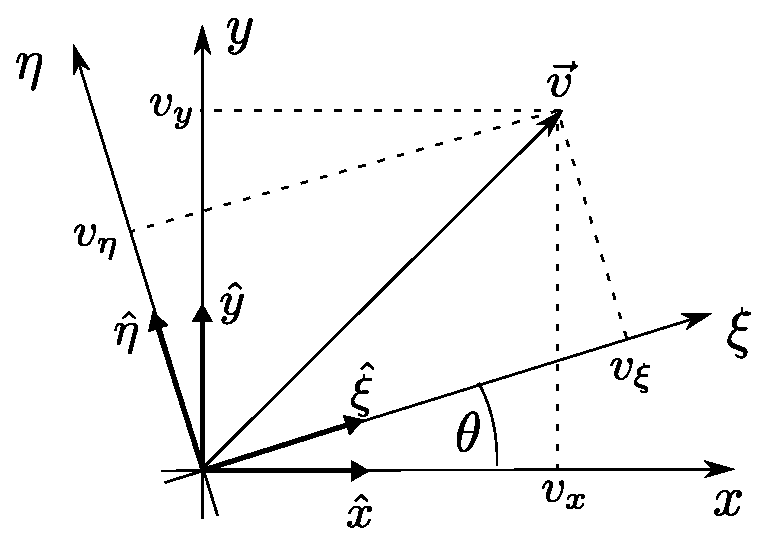
\includegraphics[width=0.95\textwidth]{./fig/rotation}
\end{center}
\end{minipage}
\end{tabular}
 
 
 
 
 
 
 
 
 
 
 



 \paragraph{Osservazione.}
 Gli elementi della base e le componenti di un vettore si trasformano seguendo le regole
 \begin{equation}
 \begin{cases}
  \tilde{\bm{e}}_i = \hat{T}^k_i \bm{e}_k  = \hat{T}_{ik} \bm{e}_k = T_{ki} \bm{e}_k\\
  \tilde{v}^i      = T^i_k v^k             = T_{ki} v^k            = \hat{T}_{ik} v^k
 \end{cases}
 \label{eqn:trGen}
 \end{equation}
 Come giustamente osservato da alcuni di voi, i vettori delle basi e le componenti dei vettori
 seguono la stessa trasformazione: questo è vero nel caso di rotazioni, poichè $\hat{T}:=T^{-1}=T^T$,
 in componenti $\hat{T}_{ik} = T_{ki}$ (osservate le relazioni qui sopra (\ref{eqn:trGen}) e come questo implica
 l'uguaglianza delle trasformazioni dei vettori della base e delle componenti). 
 Dalle relazioni trovate è immediato ricavare le trasformazioni inverse
 \begin{equation}
 \begin{cases}
  \bm{e}_i = T_{ik} \tilde{\bm{e}}_k = \hat{T}_{ki} \tilde{\bm{e}}_k\\
  v^i      = T_{ik} \tilde{v}^k      = \hat{T}_{ki} \tilde{v}^k
 \end{cases}
 \end{equation}
 
 \noindent
 Quando lo spazio è di dimensione 2, come nel nostro esercizio, si possono esplicitare le trasformazioni
 (\ref{eqn:trGen})
 
 \begin{equation}
 \begin{cases}
  \tilde{\bm{e}}_1 =  \hat{T}_{11} \bm{e}_1 + \hat{T}_{12} \bm{e}_2 \\
  \tilde{\bm{e}}_2 =  \hat{T}_{21} \bm{e}_1 + \hat{T}_{22} \bm{e}_2 \\
 \end{cases}
 \qquad
 \begin{cases}
  \tilde{v}_1 =  \hat{T}_{11} v_1 + \hat{T}_{12} v_2 \\
  \tilde{v}_2 =  \hat{T}_{21} v_1 + \hat{T}_{22} v_2 \\
 \end{cases}
 \label{eqn:trGen2}
 \end{equation}
 
 \vspace{0.05cm}
 \begin{center}
 \rule{0.75\textwidth}{.4pt}
 \end{center}
 \vspace{0.2cm}
 
 Si torna all'esercizio per ricavare la matrice di rotazione $T$, con le convezioni usate nell'osservazione, sostituendo
 al sistema indicato con la tilde il sistema $(\xi,\eta)$.
 Confrontando le trasformazioni (\ref{eqn:trEse}) dell'esercizio con quelle generali (\ref{eqn:trGen2}),
 la matrice di rotazione $\hat{T}$ che fa passare da $(x,y)$ a $(\xi,\eta)$ e la sua 
 inversa  $T$ (che coincide con la trasposta) sono
 \begin{equation}
 \hat{T} = \begin{bmatrix} 
  \cos{\theta} & \sin{\theta} \\
 -\sin{\theta} & \cos{\theta} \\
 \end{bmatrix}
 \qquad
 T = \begin{bmatrix} 
  \cos{\theta} & -\sin{\theta} \\
  \sin{\theta} &  \cos{\theta} \\
 \end{bmatrix}
 \end{equation}
 
 Consideriamo ora un tensore $\bm{A}$ del secondo ordine. Un esempio di tensore del secondo ordine è il tensore degli sforzi, 
 che ha anche la proprietà di essere simmetrico, $A_{ij} = A_{ji}$. Si può scrivere il tensore $\bm{A}$ in componenti rispetto alle due basi

 \begin{equation}
 \begin{aligned}
  \bm{A} & = A_{kl} \bm{e}_k \otimes \bm{e}_l = \\
   & = {A}_{kl} \hat{T}_{ik} \hat{T}_{jl} \tilde{\bm{e}}_i \otimes \tilde{\bm{e}}_j \\
   & = \tilde{A}_{ij} \tilde{\bm{e}}_i \otimes \tilde{\bm{e}}_j \\
 \end{aligned}
 \end{equation}
 
 Ragionando sugli indici, ricordando che indici ripetuti si sommano, è possibile rappresentare la trasformazione
 $\tilde{A}_{ij} = {A}_{kl} \hat{T}_{ik} \hat{T}_{jl}$
 delle componenti di un tensore del secondo ordine in forma matriciale
 \begin{equation}
 \begin{aligned}
   \tilde{A} & = \hat{T} A \hat{T}^T = T^T A T \\
   A & = \hat{T}^T \tilde{A} \hat{T} = T \tilde{A} T^T \\
 \label{eqn:trasfT2}
 \end{aligned}
 \end{equation}
 dove si sono definite le matrici $A$, $\tilde{A}$ contenti le componenti $A_{ij}$, $\tilde{A}_{ij}$ con il primo
  indice indicante la riga, il secondo la colonna.
  
 Il tensore $\bm{A}$ dell'esempio può essere scritto esplicitando tutti termini come
 \begin{equation}
 \begin{aligned}
  \bm{A} & = A_{xx} \bm{\hat{x}} \otimes \bm{\hat{x}} + A_{xy} \bm{\hat{x}} \otimes \bm{\hat{y}} 
           + A_{yx} \bm{\hat{y}} \otimes \bm{\hat{x}} + A_{yy} \bm{\hat{y}} \otimes \bm{\hat{y}} = \\
         & = A_{\xi\xi} \bm{\hat{\xi}} \otimes \bm{\hat{\xi}} + A_{\xi\eta} \bm{\hat{\xi}} \otimes \bm{\hat{\eta}} 
           + A_{\eta\xi} \bm{\hat{\eta}} \otimes \bm{\hat{\xi}} + A_{\eta\eta} \bm{\hat{\eta}} \otimes \bm{\hat{\eta}}
 \end{aligned}
 \end{equation}
 
 Le quattro componenti in ciascuna delle due basi possono essere organizzate in due matrici, legate tra di loro
 dalla relazione (\ref{eqn:trasfT2})
 \begin{equation}
   \begin{bmatrix}
    A_{\xi \xi} & A_{\xi \eta} \\
    A_{\eta\xi} & A_{\eta\eta} \\
   \end{bmatrix} = 
   \begin{bmatrix} 
    \cos{\theta} &-\sin{\theta} \\
    \sin{\theta} & \cos{\theta} \\
   \end{bmatrix}
   \begin{bmatrix}
    A_{xx} & A_{xy} \\
    A_{yx} & A_{yy} \\
   \end{bmatrix}
   \begin{bmatrix} 
    \cos{\theta} & \sin{\theta} \\
   -\sin{\theta} & \cos{\theta} \\
   \end{bmatrix}
 \end{equation}
 
 \paragraph{Tensore degli sforzi, sforzo piano e direzioni principali.}
Vediamo ora un esempio pratico, ingegneristico, di quanto fatto fino ad ora.
 Durante il corso di Scienze delle costruzioni avete incontrato il cerchio di Mohr, utilizzabile in uno stato di sforzo piano 
 ($\tau_{xz} = \sigma_{xz} = 0$, $\tau_{yz} = \sigma_{yz} = 0$, $\sigma_{zz} = 0$) per
\begin{itemize}
 \item trovare il vettore sforzo agente su una superficie di normale $\bm{\hat{n}}$, noto il tensore degli sforzi
 \item trovare gli sforzi principali e le direzioni principali (per le quali le componenti di taglio sono nulle)
\end{itemize}
 Cerchiamo ora di trovare le direzioni principali (basta trovare una direzione, l'altra è perpendicolare, poichè il tensore
 è simmetrico, $A_{xy} = A_{yx}$), usando la trasformazione appena trovata per un tensore simmetrico $\bm{A}$.
  \begin{equation}
  \begin{aligned}
   \begin{bmatrix}
    A_{\xi \xi} & A_{\xi \eta} \\
    A_{\eta\xi} & A_{\eta\eta} \\
   \end{bmatrix} & = 
   \begin{bmatrix} 
    \cos{\theta} & \sin{\theta} \\
   -\sin{\theta} & \cos{\theta} \\
   \end{bmatrix}
   \begin{bmatrix}
    A_{xx} & A_{xy} \\
    A_{xy} & A_{yy} \\
   \end{bmatrix}
   \begin{bmatrix} 
    \cos{\theta} &-\sin{\theta} \\
   \sin{\theta} & \cos{\theta} \\
   \end{bmatrix} = \\
   & = \begin{bmatrix}
    A_{xx} \cos^2 \theta + A_{yy} \sin^2 \theta + 2 A_{xy} \cos \theta \sin \theta & 
      (-A_{xx} + A_{yy}) \cos \theta \sin \theta + A_{xy} ( \cos^2 \theta - \sin^2 \theta) \\
  (-A_{xx} + A_{yy}) \cos \theta \sin \theta + A_{xy} ( \cos^2 \theta - \sin^2 \theta) &
      A_{xx} \sin^2 \theta + A_{yy} \cos^2 \theta - 2 A_{xy} \cos \theta \sin \theta 
   \end{bmatrix}
 \end{aligned}
 \end{equation}
 La proprietà di simmetria del tensore è indipendente dal sistema di coordinate nel quale vengono scritte le componenti
  ($A_{\xi \eta} = A_{\eta \xi}$).
  Per trovare l'angolo del quale sono ruotati gli assi principali rispetto agli assi $(x,y)$ imponiamo che si annulli la
  componente fuori dalla diagonale nel sistema ruotato
  \begin{equation}
   A_{\xi \eta} = 0
  \end{equation}
  \begin{equation}
   0 = A_{xy} \cos {2\theta} - \dfrac{\sin{2\theta}}{2} (A_{xx}-A_{yy}) \quad \Rightarrow \quad
   \tan {2 \theta} = \dfrac{2 A_{xy}}{A_{xx}-A_{yy}}
  \end{equation}
 %
 Il problema oggetto di questo esercizio è equivalente alla ricerca degli assi principali di sforzo per uno stato di sforzo piano.
  Il risultato ricavato tramite le trasformazioni delle componenti dei tensori coincide con quello  già ottenuto nei corsi precedenti tramite l'equilibrio di un elementino di materiale, riassumibile nel diagramma del cerchio di Mohr. Avere in mente entrambi gli approcci è utile per non perdere il significato fisico di quello che si sta facendo.
 \newline \noindent 
  Un altro impiego della trasformazione precedente, sempre ``da strutturista'', un po' più avanzato, è la determinazione 
  delle caratteristiche di elementi di materiale in composito, partendo dalle proprietà delle lamine che vengono 
  usate per costruirlo.
  Le lamine hanno caratteristiche espresse nel proprio sistema di riferimento, che in generale ha orientazione diversa
  da lamina a lamina, e diversa da un sistema di riferimento per l'elemento strutturale.
 \newline \noindent 
 Queste poche righe non hanno pretese di completezza, ma vogliono attirare l'interesse su quanto abbiamo visto nelle ultime 4 ore,
  anche da parte di quelli che diventeranno ``strutturisti'' ma non solo.
  
